\documentclass{standalone}
\usepackage{tikz}
\usetikzlibrary{patterns, positioning}

\begin{document}
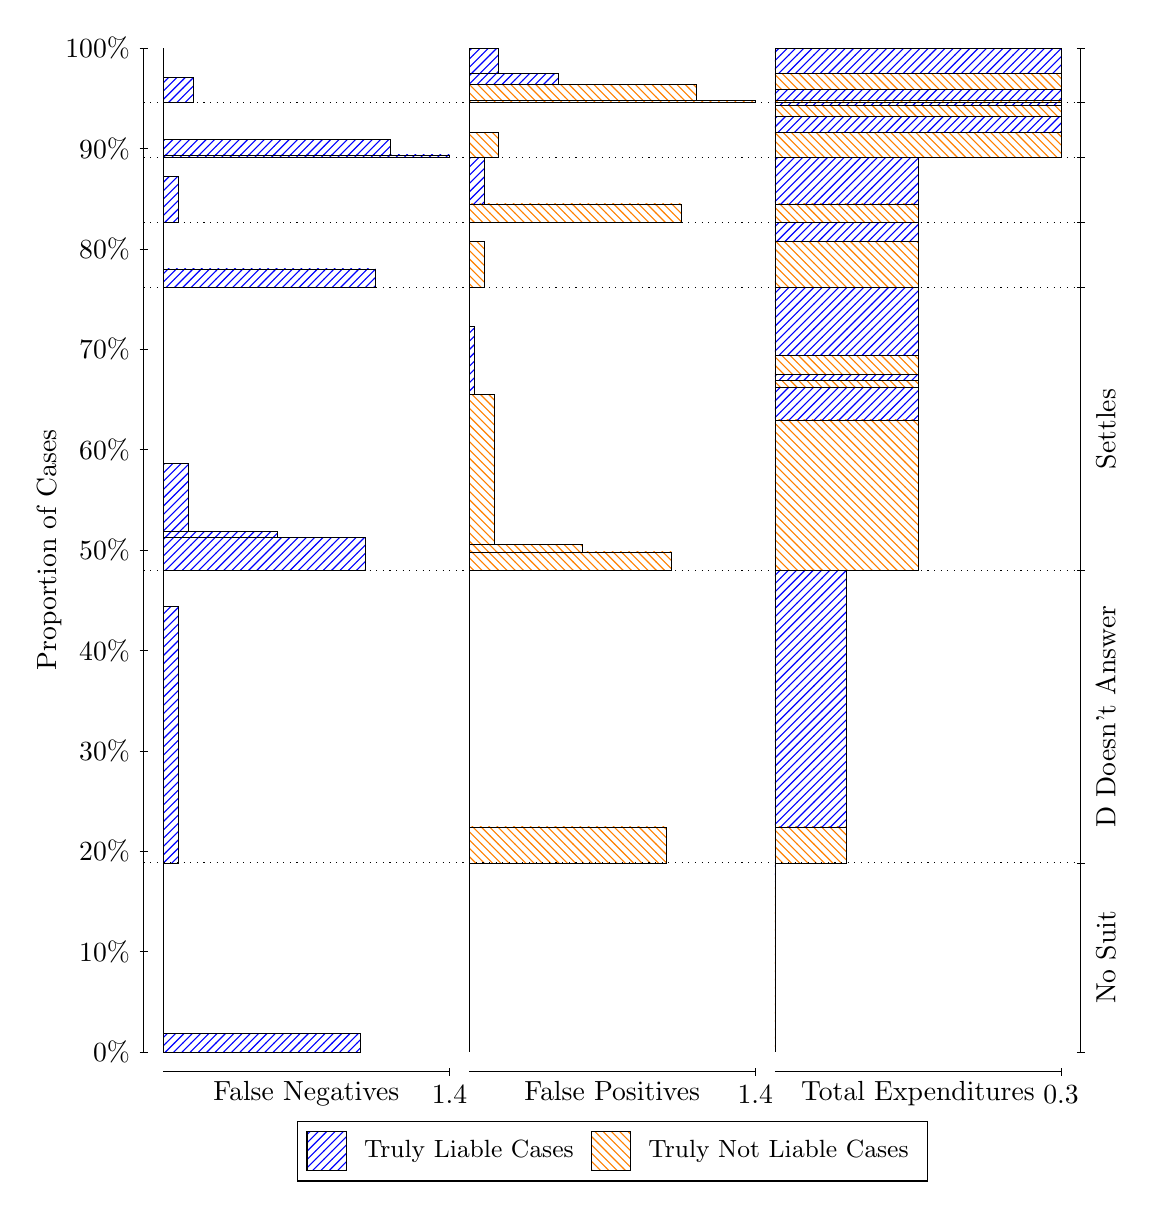
\begin{tikzpicture}
\draw[black, very thin] (1.5,1.75) -- (1.5,14.5);
\node[rotate=90, anchor=center] at (0.3, 8.125) {Proportion of Cases};
\draw[black, very thin] (1.45,1.75) -- (1.55,1.75);
\node[anchor=east] at (1.45, 1.75) {0\%};
\draw[black, very thin] (1.45,3.025) -- (1.55,3.025);
\node[anchor=east] at (1.45, 3.025) {10\%};
\draw[black, very thin] (1.45,4.3) -- (1.55,4.3);
\node[anchor=east] at (1.45, 4.3) {20\%};
\draw[black, very thin] (1.45,5.575) -- (1.55,5.575);
\node[anchor=east] at (1.45, 5.575) {30\%};
\draw[black, very thin] (1.45,6.85) -- (1.55,6.85);
\node[anchor=east] at (1.45, 6.85) {40\%};
\draw[black, very thin] (1.45,8.125) -- (1.55,8.125);
\node[anchor=east] at (1.45, 8.125) {50\%};
\draw[black, very thin] (1.45,9.4) -- (1.55,9.4);
\node[anchor=east] at (1.45, 9.4) {60\%};
\draw[black, very thin] (1.45,10.675) -- (1.55,10.675);
\node[anchor=east] at (1.45, 10.675) {70\%};
\draw[black, very thin] (1.45,11.95) -- (1.55,11.95);
\node[anchor=east] at (1.45, 11.95) {80\%};
\draw[black, very thin] (1.45,13.225) -- (1.55,13.225);
\node[anchor=east] at (1.45, 13.225) {90\%};
\draw[black, very thin] (1.45,14.5) -- (1.55,14.5);
\node[anchor=east] at (1.45, 14.5) {100\%};

\draw[black, very thin] (13.4,1.75) -- (13.4,14.5);
\draw[black, very thin] (13.35,1.75) -- (13.45,1.75);
\node[anchor=west] at (13.35, 1.75) {};
\draw[black, very thin] (13.35,4.1507) -- (13.45,4.1507);
\node[anchor=west] at (13.35, 4.1507) {};
\draw[black, very thin] (13.35,7.8663) -- (13.45,7.8663);
\node[anchor=west] at (13.35, 7.8663) {};
\draw[black, very thin] (13.35,11.456) -- (13.45,11.456);
\node[anchor=west] at (13.35, 11.456) {};
\draw[black, very thin] (13.35,12.283) -- (13.45,12.283);
\node[anchor=west] at (13.35, 12.283) {};
\draw[black, very thin] (13.35,13.11) -- (13.45,13.11);
\node[anchor=west] at (13.35, 13.11) {};
\draw[black, very thin] (13.35,13.805) -- (13.45,13.805);
\node[anchor=west] at (13.35, 13.805) {};
\draw[black, very thin] (13.35,14.5) -- (13.45,14.5);
\node[anchor=west] at (13.35, 14.5) {};

\draw[black, very thin, pattern color=blue, pattern=north east lines] (1.75,1.75) rectangle (4.2557,1.991);
\draw[black, very thin, pattern color=orange, pattern=north west lines] (1.75,1.991) rectangle (1.75,4.1507);
\draw[black, very thin, pattern color=blue, pattern=north east lines] (1.75,4.1507) rectangle (1.9379,7.4086);
\draw[black, very thin, pattern color=orange, pattern=north west lines] (1.75,7.4086) rectangle (1.75,7.8663);
\draw[black, very thin, pattern color=blue, pattern=north east lines] (1.75,7.8663) rectangle (4.3184,8.2803);
\draw[black, very thin, pattern color=blue, pattern=north east lines] (1.75,8.2803) rectangle (3.1908,8.3576);
\draw[black, very thin, pattern color=blue, pattern=north east lines] (1.75,8.3576) rectangle (2.0632,9.2201);
\draw[black, very thin, pattern color=orange, pattern=north west lines] (1.75,9.2201) rectangle (1.75,11.456);
\draw[black, very thin, pattern color=blue, pattern=north east lines] (1.75,11.456) rectangle (4.4437,11.695);
\draw[black, very thin, pattern color=orange, pattern=north west lines] (1.75,11.695) rectangle (1.75,12.283);
\draw[black, very thin, pattern color=blue, pattern=north east lines] (1.75,12.283) rectangle (1.9379,12.87);
\draw[black, very thin, pattern color=orange, pattern=north west lines] (1.75,12.87) rectangle (1.75,13.11);
\draw[black, very thin, pattern color=blue, pattern=north east lines] (1.75,13.11) rectangle (5.3833,13.144);
\draw[black, very thin, pattern color=blue, pattern=north east lines] (1.75,13.144) rectangle (4.6316,13.343);
\draw[black, very thin, pattern color=orange, pattern=north west lines] (1.75,13.343) rectangle (1.75,13.805);
\draw[black, very thin, pattern color=blue, pattern=north east lines] (1.75,13.805) rectangle (2.1259,14.129);
\draw[black, very thin, pattern color=orange, pattern=north west lines] (1.75,14.129) rectangle (1.75,14.362);
\draw[black, very thin, pattern color=blue, pattern=north east lines] (1.75,14.362) rectangle (1.75,14.5);
\draw[black, very thin, pattern color=orange, pattern=north west lines] (5.6333,1.75) rectangle (5.6333,3.9097);
\draw[black, very thin, pattern color=blue, pattern=north east lines] (5.6333,3.9097) rectangle (5.6333,4.1507);
\draw[black, very thin, pattern color=orange, pattern=north west lines] (5.6333,4.1507) rectangle (8.1391,4.6084);
\draw[black, very thin, pattern color=blue, pattern=north east lines] (5.6333,4.6084) rectangle (5.6333,7.8663);
\draw[black, very thin, pattern color=orange, pattern=north west lines] (5.6333,7.8663) rectangle (8.2017,8.1009);
\draw[black, very thin, pattern color=orange, pattern=north west lines] (5.6333,8.1009) rectangle (7.0741,8.1915);
\draw[black, very thin, pattern color=orange, pattern=north west lines] (5.6333,8.1915) rectangle (5.9466,10.102);
\draw[black, very thin, pattern color=blue, pattern=north east lines] (5.6333,10.102) rectangle (5.696,10.964);
\draw[black, very thin, pattern color=blue, pattern=north east lines] (5.6333,10.964) rectangle (5.6333,11.456);
\draw[black, very thin, pattern color=orange, pattern=north west lines] (5.6333,11.456) rectangle (5.8213,12.043);
\draw[black, very thin, pattern color=blue, pattern=north east lines] (5.6333,12.043) rectangle (5.6333,12.283);
\draw[black, very thin, pattern color=orange, pattern=north west lines] (5.6333,12.283) rectangle (8.327,12.522);
\draw[black, very thin, pattern color=blue, pattern=north east lines] (5.6333,12.522) rectangle (5.8213,13.11);
\draw[black, very thin, pattern color=orange, pattern=north west lines] (5.6333,13.11) rectangle (6.0092,13.433);
\draw[black, very thin, pattern color=orange, pattern=north west lines] (5.6333,13.433) rectangle (5.6333,13.572);
\draw[black, very thin, pattern color=blue, pattern=north east lines] (5.6333,13.572) rectangle (5.6333,13.805);
\draw[black, very thin, pattern color=orange, pattern=north west lines] (5.6333,13.805) rectangle (9.2667,13.839);
\draw[black, very thin, pattern color=orange, pattern=north west lines] (5.6333,13.839) rectangle (8.5149,14.038);
\draw[black, very thin, pattern color=blue, pattern=north east lines] (5.6333,14.038) rectangle (6.7609,14.176);
\draw[black, very thin, pattern color=blue, pattern=north east lines] (5.6333,14.176) rectangle (6.0092,14.5);
\draw[black, very thin, pattern color=orange, pattern=north west lines] (9.5167,1.75) rectangle (9.5167,3.9097);
\draw[black, very thin, pattern color=blue, pattern=north east lines] (9.5167,3.9097) rectangle (9.5167,4.1507);
\draw[black, very thin, pattern color=orange, pattern=north west lines] (9.5167,4.1507) rectangle (10.425,4.6084);
\draw[black, very thin, pattern color=blue, pattern=north east lines] (9.5167,4.6084) rectangle (10.425,7.8663);
\draw[black, very thin, pattern color=orange, pattern=north west lines] (9.5167,7.8663) rectangle (11.333,9.7767);
\draw[black, very thin, pattern color=blue, pattern=north east lines] (9.5167,9.7767) rectangle (11.333,10.191);
\draw[black, very thin, pattern color=orange, pattern=north west lines] (9.5167,10.191) rectangle (11.333,10.281);
\draw[black, very thin, pattern color=blue, pattern=north east lines] (9.5167,10.281) rectangle (11.333,10.359);
\draw[black, very thin, pattern color=orange, pattern=north west lines] (9.5167,10.359) rectangle (11.333,10.593);
\draw[black, very thin, pattern color=blue, pattern=north east lines] (9.5167,10.593) rectangle (11.333,11.456);
\draw[black, very thin, pattern color=orange, pattern=north west lines] (9.5167,11.456) rectangle (11.333,12.043);
\draw[black, very thin, pattern color=blue, pattern=north east lines] (9.5167,12.043) rectangle (11.333,12.283);
\draw[black, very thin, pattern color=orange, pattern=north west lines] (9.5167,12.283) rectangle (11.333,12.522);
\draw[black, very thin, pattern color=blue, pattern=north east lines] (9.5167,12.522) rectangle (11.333,13.11);
\draw[black, very thin, pattern color=orange, pattern=north west lines] (9.5167,13.11) rectangle (13.15,13.433);
\draw[black, very thin, pattern color=blue, pattern=north east lines] (9.5167,13.433) rectangle (13.15,13.632);
\draw[black, very thin, pattern color=orange, pattern=north west lines] (9.5167,13.632) rectangle (13.15,13.77);
\draw[black, very thin, pattern color=blue, pattern=north east lines] (9.5167,13.77) rectangle (13.15,13.805);
\draw[black, very thin, pattern color=orange, pattern=north west lines] (9.5167,13.805) rectangle (13.15,13.839);
\draw[black, very thin, pattern color=blue, pattern=north east lines] (9.5167,13.839) rectangle (13.15,13.978);
\draw[black, very thin, pattern color=orange, pattern=north west lines] (9.5167,13.978) rectangle (13.15,14.176);
\draw[black, very thin, pattern color=blue, pattern=north east lines] (9.5167,14.176) rectangle (13.15,14.5);
\draw[black, dotted] (1.5,4.1507) -- (13.4,4.1507);
\draw[black, dotted] (1.5,7.8663) -- (13.4,7.8663);
\draw[black, dotted] (1.5,11.456) -- (13.4,11.456);
\draw[black, dotted] (1.5,12.283) -- (13.4,12.283);
\draw[black, dotted] (1.5,13.11) -- (13.4,13.11);
\draw[black, dotted] (1.5,13.805) -- (13.4,13.805);
\draw[black, very thin] (1.75,1.5) -- (5.3833,1.5);
\node[anchor=north] at (3.5667, 1.5) {False Negatives};
\draw[black, very thin] (5.3833,1.45) -- (5.3833,1.55);
\node[anchor=north] at (5.3833, 1.45) {1.4};

\draw[black, very thin] (5.6333,1.5) -- (9.2667,1.5);
\node[anchor=north] at (7.45, 1.5) {False Positives};
\draw[black, very thin] (9.2667,1.45) -- (9.2667,1.55);
\node[anchor=north] at (9.2667, 1.45) {1.4};

\draw[black, very thin] (9.5167,1.5) -- (13.15,1.5);
\node[anchor=north] at (11.333, 1.5) {Total Expenditures};
\draw[black, very thin] (13.15,1.45) -- (13.15,1.55);
\node[anchor=north] at (13.15, 1.45) {0.3};

\node[black, centered, rotate=90] at (13.72, 2.9503) {No Suit};
\node[black, centered, rotate=90] at (13.72, 6.0085) {D Doesn't Answer};
\node[black, centered, rotate=90] at (13.72, 9.661) {Settles};





\draw (7.449999999999999,1.5) node[draw=none] (baseCoordinate) {};
\begin{scope}[align=center]
        \matrix[scale=0.5, draw=black, below=0.5cm of baseCoordinate, nodes={draw}, column sep=0.1cm]{
            \node[rectangle, draw, minimum width=0.5cm, minimum height=0.5cm, pattern=north east lines, pattern color=blue] {}; &
            \node[draw=none, font=\small] (B) {Truly Liable Cases}; &
            \node[rectangle, draw, minimum width=0.5cm, minimum height=0.5cm, pattern=north west lines, pattern color=orange] {}; &
            \node[draw=none, font=\small] (B) {Truly Not Liable Cases}; \\
            };
\end{scope}

\end{tikzpicture}
\end{document}